\chapter{Design} \label{section:design}
In the spirit of an extensive overview of standardized procedures of industrial vibration acquisition and monitoring, the methods in feature selection, feature selection, and machine diagnostics from vibration signals, we propose a preliminary design of elements in the sensor network capable of discriminating machinery faults.

\section{Machine learning pipeline}

Mafaulda dataset
Jupyter notebook - Python
\begin{enumerate}
    \itemsep0pt
    \item Detrending
    \item (Optional) Adaptive noise cancellation of the background interference
    \item Vector of all features
    \begin{itemize}
        \itemsep0pt
        \item Time domain: statistical measures (Tab.~\ref{tab:td-features})
        \item Frequency domain: PSD estimation with FFT and Welch averaging with the resolution of 1 Hz combined with Hann window (Tab.~\ref{tab:fd-features})
    \end{itemize}
    \item Feature selection on evaluation datasets and experimental measurements from the factory to prune away irrelevant features with pearson correlation, Fisher score, and mutal information.
    \item Model evaluation and comparison of novelty detection methods and precision of classification with different sets of predictors. The range of optimal parameters will be found for the DenStream ($\mu$, $\epsilon$, $beta$, $\lambda$), Half-Space Trees (window size, ensemble size), and kNN (distance metric, $k$ neighbours). Evaluation metrics associated with confusion matrices will be used like accuracy, precision, true positive rate, and false positive rate.
\end{enumerate}

\begin{figure}[h]
\centering
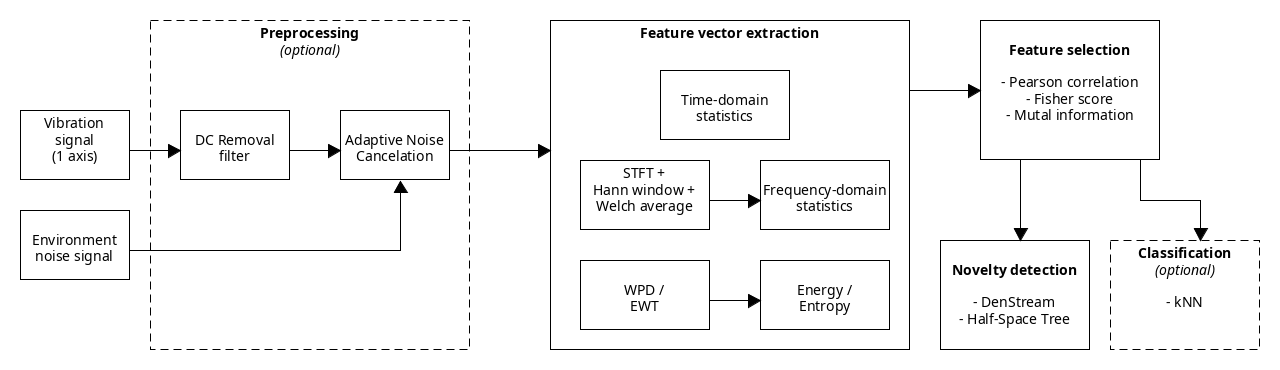
\includegraphics[width=0.9\textwidth]{assets/ml-lifecycle.png}
\caption{Machine learning lifecycle of feature discovery}
\end{figure}


\section{Research questions}
Open ended Research questions:
	- Which time and frequency features can be extracted from vibrational signals to provide an accurate record of machinery faults?
	- What are the savings in transmission bandwidth when chosen signal features are used in comparison to raw sampled measurement or lossless compression techniques?
	- How can the machinery faults be continuously identified based on collected events?

Main goals:
	- How does vibration data look like (spectral and time domain)?
	- Create dataset of machinery vibrations
	- Reduce number of features (samples) send from edge device - to minimal amount
	- Adapt to features changing over time (RiverML can handle it, find proof)
	- Evaluate model performance on all features and different feature sets
	- Keep in mind: data ordering!

\section{Data preparation}
- Machinery:
   - KALORIK BASIC Stand Fan TKGVT1037C  - height 125 cm, stable 60 cm cross base, 3 speed, 45 W, 45 cm fan diameter, 3 propelers
   - AC unit VERTIV: Scroll Compressor: Copeland ZR16M3E-TWD-561 (2900 RPM @ 50 Hz; 9.7 kW (13 HP); 380/420V; 25 A) - 2 units
   - Water pump: KSB Omega 300-560 B GB G F (2018, 1493 (1500) RPM @ 50 Hz; 500 kW elektromotor; power requirement: 380 kW) - 1 unit
   
- Sensors:
	- Accelerometer: ADXL335 ($\pm$3g, Bandwidth: 0.55 kHz)
	- Noise density: 150 - 300 $\mu g / \sqrt{Hz}$ rms
	- Resolution: 12 bits
	- Axis: 3 axis
	- Sensitvity: 300 mV/g
	- Sample time: 400 ns (2.5 kHz)
	- Voltage range: up to 1.8 V
	
	- IIS3DWB (STEVAL-MKI208V1K) Digitálny (SPI), 1 / 3 axis, Resultution: 16 bits ADC, Range: 2 - 16g, Sensitvity: 0.061 mg/LSB pri 2g, Noise density:: 75 $\mu g / \sqrt{Hz}$, ODR: 26.7 kHz,Bandwidth: 5 - 6.3 kHz (-3 dB), FIFO: 3 kB (512 vzoriek)

- EDA
	- Time waveform
	- Spectrogram
	- Features: boxplot

- Experiment subsets:
	features = temporal, spectral
	rpm_limit = False, True
	hardware = shaft, bearings
	target = fault, anomaly_60, anomaly_90
	placement = A, B
	online = False, True


- Mafaulda dataset
	- Choose 4 faults - normal (N), imbalance (I), vertical (VM) and horizonal misalignment (HM)
	- Convert severity to 0 - 1 scale.
		- Label samples above 0., 0.9 as anomalous
	- Choose rpm range 2900 $\pm$ 500 (around rotational speed of machinery with some spread, some features are correlated with rpm 
	- Counts before split: 
		- Split to 5 parts of 1 second intervals
	- Two measurement points A, B
	- Detrending by removing mean
	- Calculate features: temporal, spectral (in 5 window sizes): welch averaging, hann window
	
	- Batch: 
		- Balancing dataset with oversampling minority classes	
		- Hold-out validation - split to train and test set
	- Online: Order by severity

- Measurement of custom datasets 
	- one 3-axis accelerometer on top of scroll compressor of air conditioning
		- one in the base to capture noise
	- water pump
	
	- columns: t, x, y, z: rpm
	- 20 s recordings - split to 5 parts - extract features
	- do PCA to explore see differences
	- label as worse, better (classes are hard to provide)

- \textbf{Measurements-SHC3.html}
- \textbf{BVS-Measurements.html}

\section{Feature relevance}
- \textbf{FeatureSummary.html}

- choose 3 features
- supervised
	- highly correlated features >= 0.9:
		- Temporal domain (A)
			- std, rms, 1.000000
			- margin, impulse, 0.999079
			- crest, impulse, 0.996807
			- crest, margin,	0.992548
			- pp, max, 0.970055
			- max, (std, rms), 0.938198
			- pp, (std, rms), 0.938180 / 0.928
		- Spectral domain (A)
			- same feature in different window sizes (0.99)
			- kurtosis, skewness, 0.980618
			- std, energy, 0.960110
			- entropy, noisiness, 0.945514

	- calcultate euclidian measure of feature 
	- correlation point biserial, fisher, mutual information
		- Sperman rank correlation: corr, f\_stat, 0.98
	- calculate feature rank
		- Temporal (A) - Remove corr: pp, skewness, margin
		- Spectral (A) - multiple window sizes 
			- (energy, roll off, std) 

- online learning features
	- evolution of feature importace

\section{Nearest neighbour classifier}
- \textbf{kNN.html}
- kNN (fault and anomaly)
	- Offine (baseline)
	- Online (evolution)
- parameters: k-neigh, distance
- metrics: accuracy, precision, recall

\section{Clustering}
- Density based clustering
	- DBSCAN (all features, PCA, subset of best)
	- DenStream (all features, subset of best)

\section{Novelty detection}
- Offline (Isolation forest)
- Online (Half-space Tree)


\section{Infrastructure deployment}
Future work: engineer new feature, deploy, tweek models, validate on real dataset

 \begin{itemize}
 \itemsep0pt
\item \textbf{Input:} Samples from three-axis MEMS accelerometers, RPM tachometer, Noise background
\item \textbf{Output:} machine health status / type of fault
\item \textbf{Output on demand}: Control chart of trend features
\end{itemize}

\begin{enumerate}
\itemsep0pt
\item \textbf{Accelerometer} - MEMS accelerometers will be placed on at least two distinct measurement points in two perpendicular axes and one sensor in the machine base for denoising purposes. Rotational speed has to be captured at the same time too. The sampling frequency shall be around 2 kHz if unbalance and looseness is to be identified, and 10 kHz if bearing faults are also of interest. The range of overall rms vibrations is not expected to exceed 30 mm/s according to the vibration severity chart.
\item \textbf{Acquisition interval} - sensor units will be triggered in regular intervals (every 15 - 60 minutes) to collect vibration recordings from the band saw (or another machine of choice). The machine has to be under the same load conditions every time is recording is active. 
\item \textbf{Features} - most relevant features are computed and compared to recent measurements. If there is a statistically significant change the whole summary is sent, otherwise keep-alive notification is sent. 
\item \textbf{Wireless network} - earlier design decision has been made to establish wireless connections. Therefore, the sensor unit will send data over Wifi (IEEE 802.11), or Thread with IEEE 802.15.4 over 2.4 GHz or 868 MHz frequency bands. The application protocol shall be Constrained Application Protocol (CoAP). The messages will be encoded by Concise Binary Object Representation (CBOR) or MessagePack which provides the best compression ratio and is widely supported.
\item \textbf{Time series database} - stores history of trend values. Raw vibration measurements can be requested by the operator at any time but are available and delayed according to transfer speeds and other network constraints. The promissing database technologies is TimescaleDB.
\item \textbf{Diagnosis panel} - continuously updates the anomaly detection and classification models with the introduction of annotations to notify the operator about observed faults and imminent failure of the machine. The dashboard is provided to display the current status of multiple machines.
\end{enumerate}

\begin{figure}[h]
\centering
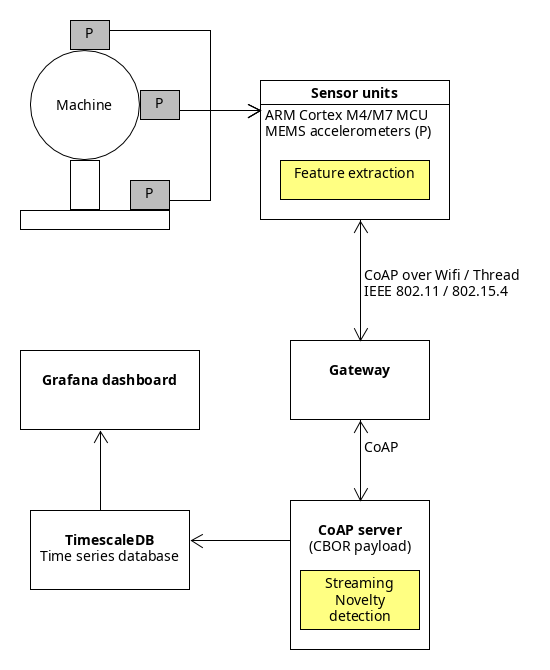
\includegraphics[width=0.7\textwidth]{assets/sensor-network.png}
\caption{Sensor network components}
\end{figure}
